
\documentclass[12pt]{article}
\usepackage{geometry} % see geometry.pdf on how to lay out the page. There's lots.
\geometry{a4paper} % or letter or a5paper or ... etc
% \geometry{landscape} % rotated page geometry
\usepackage{graphicx}
% See the ``Article customise'' template for come common customisations
\usepackage{amsmath}
\title{2D Tolerance Analysis}
\author{Ziqi Wang}
\date{} % delete this line to display the current date
\newcommand{\bt}{\mathbf{t}}
\newcommand{\bn}{\mathbf{n}}
\newcommand{\bq}{\mathbf{q}}
\newcommand{\bp}{\mathbf{p}}
\newcommand{\bc}{\mathbf{c}}
\newcommand{\tq}{\mathbf{\hat{q}}}
\newcommand{\tp}{\mathbf{\hat{p}}}
\newcommand{\barq}{\mathbf{\bar{q}}}
\newcommand{\barp}{\mathbf{\bar{p}}}
\newcommand{\br}{\mathbf{r}}
\newcommand{\bv}{\mathbf{v}}
\newcommand{\diff}{\text{d}}
%%% BEGIN DOCUMENT
\begin{document}
\maketitle
\section{Description}
Error happens everywhere in manufacture. Especially during assembling process, overlarge items are usually hard to be fitted into the assembly. One common solution would be adding tolerance within connected parts. (show in Fig.\ref{fig:tolerance_holes}(a), each triangles is shrunk by 90\%). However, gaps or even holes appear inside the assembly (shows in Fig.\ref{fig:tolerance_holes}(b)). More importantly, gap accumulation is recognised as a non-linear progress. This paper imposes a methodology to analysis the gap accumulation in 2D.
\begin{figure}[!htbp]
  \centering
    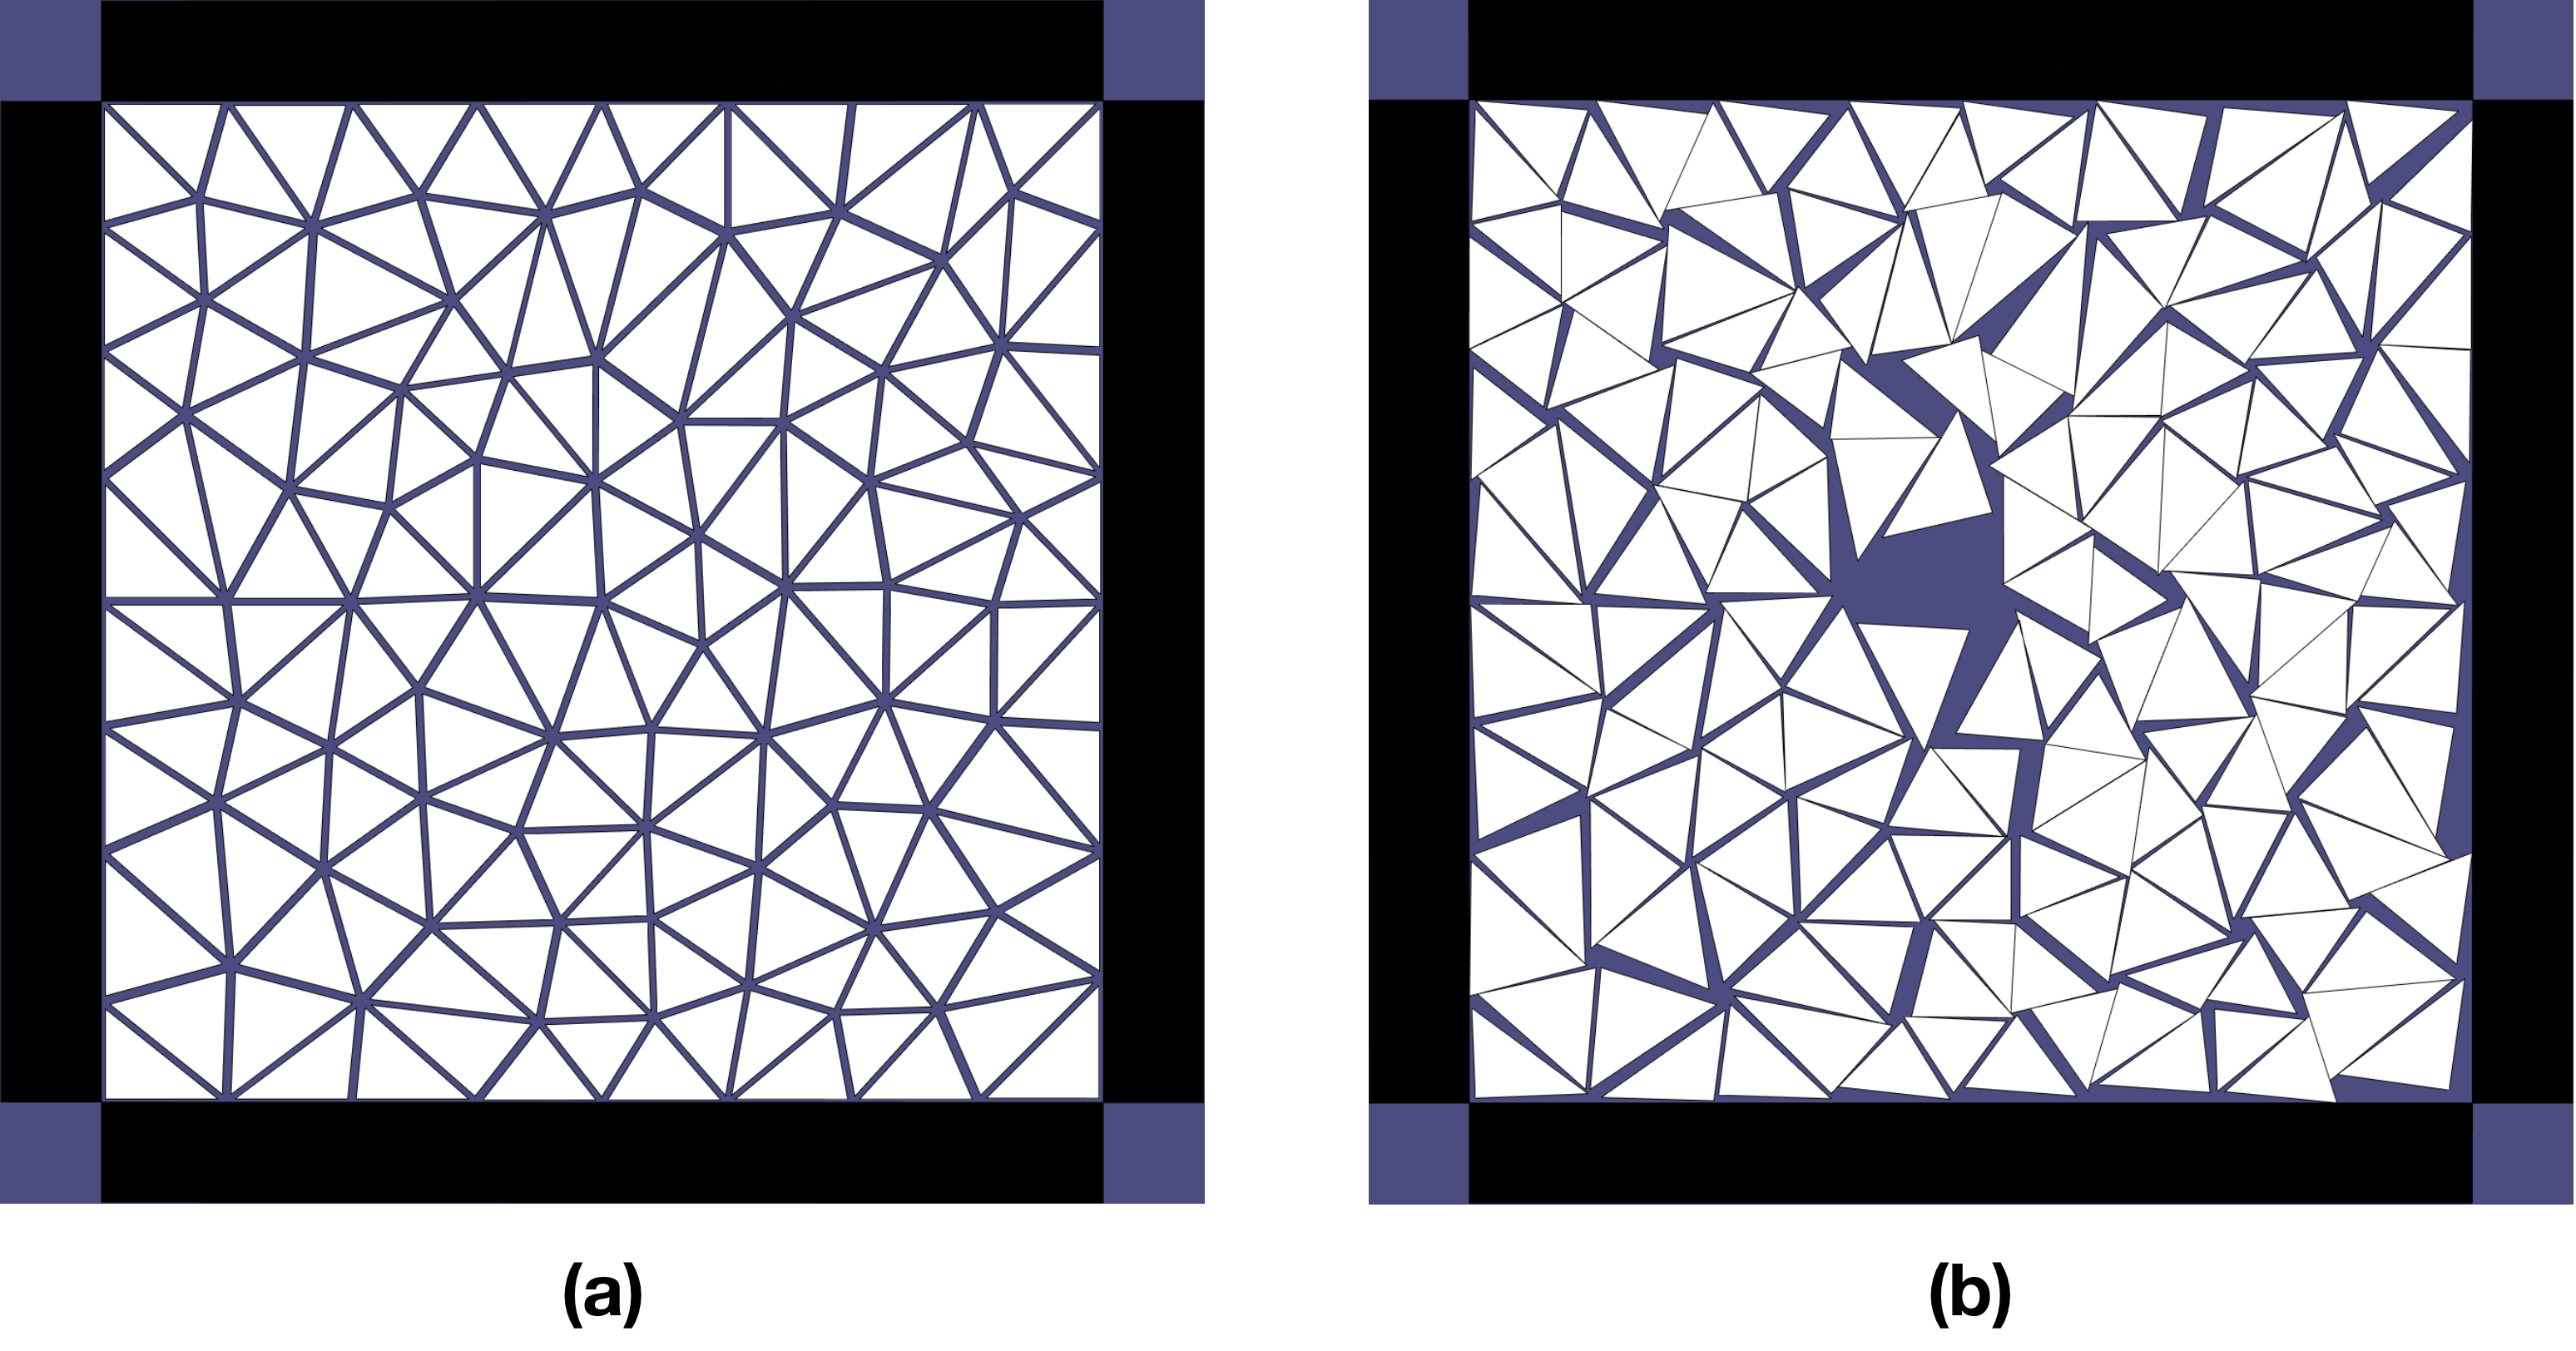
\includegraphics[width=0.6\textwidth]{ppt/tolerance_holes.png}
      \caption{Triangles (white) in (a) are shrunk and restricted by the boundary (black). To enlarge the gap among the triangles, optimizing triangles' position as well as its orientation. (b) shows triangles' layout after optimization. }
      \label{fig:tolerance_holes}
\end{figure}
\section{Methodology}
\subsection{Signed distance}
Before proposing the optimization method, we firstly define the signed distance between two polygons $P, Q$ as Fig.\ref{fig:signed_distance}. If collision happens, the signed distance $d(P, Q)$ should be smaller than $0$.\par
\begin{figure}[!htbp]
  \centering
    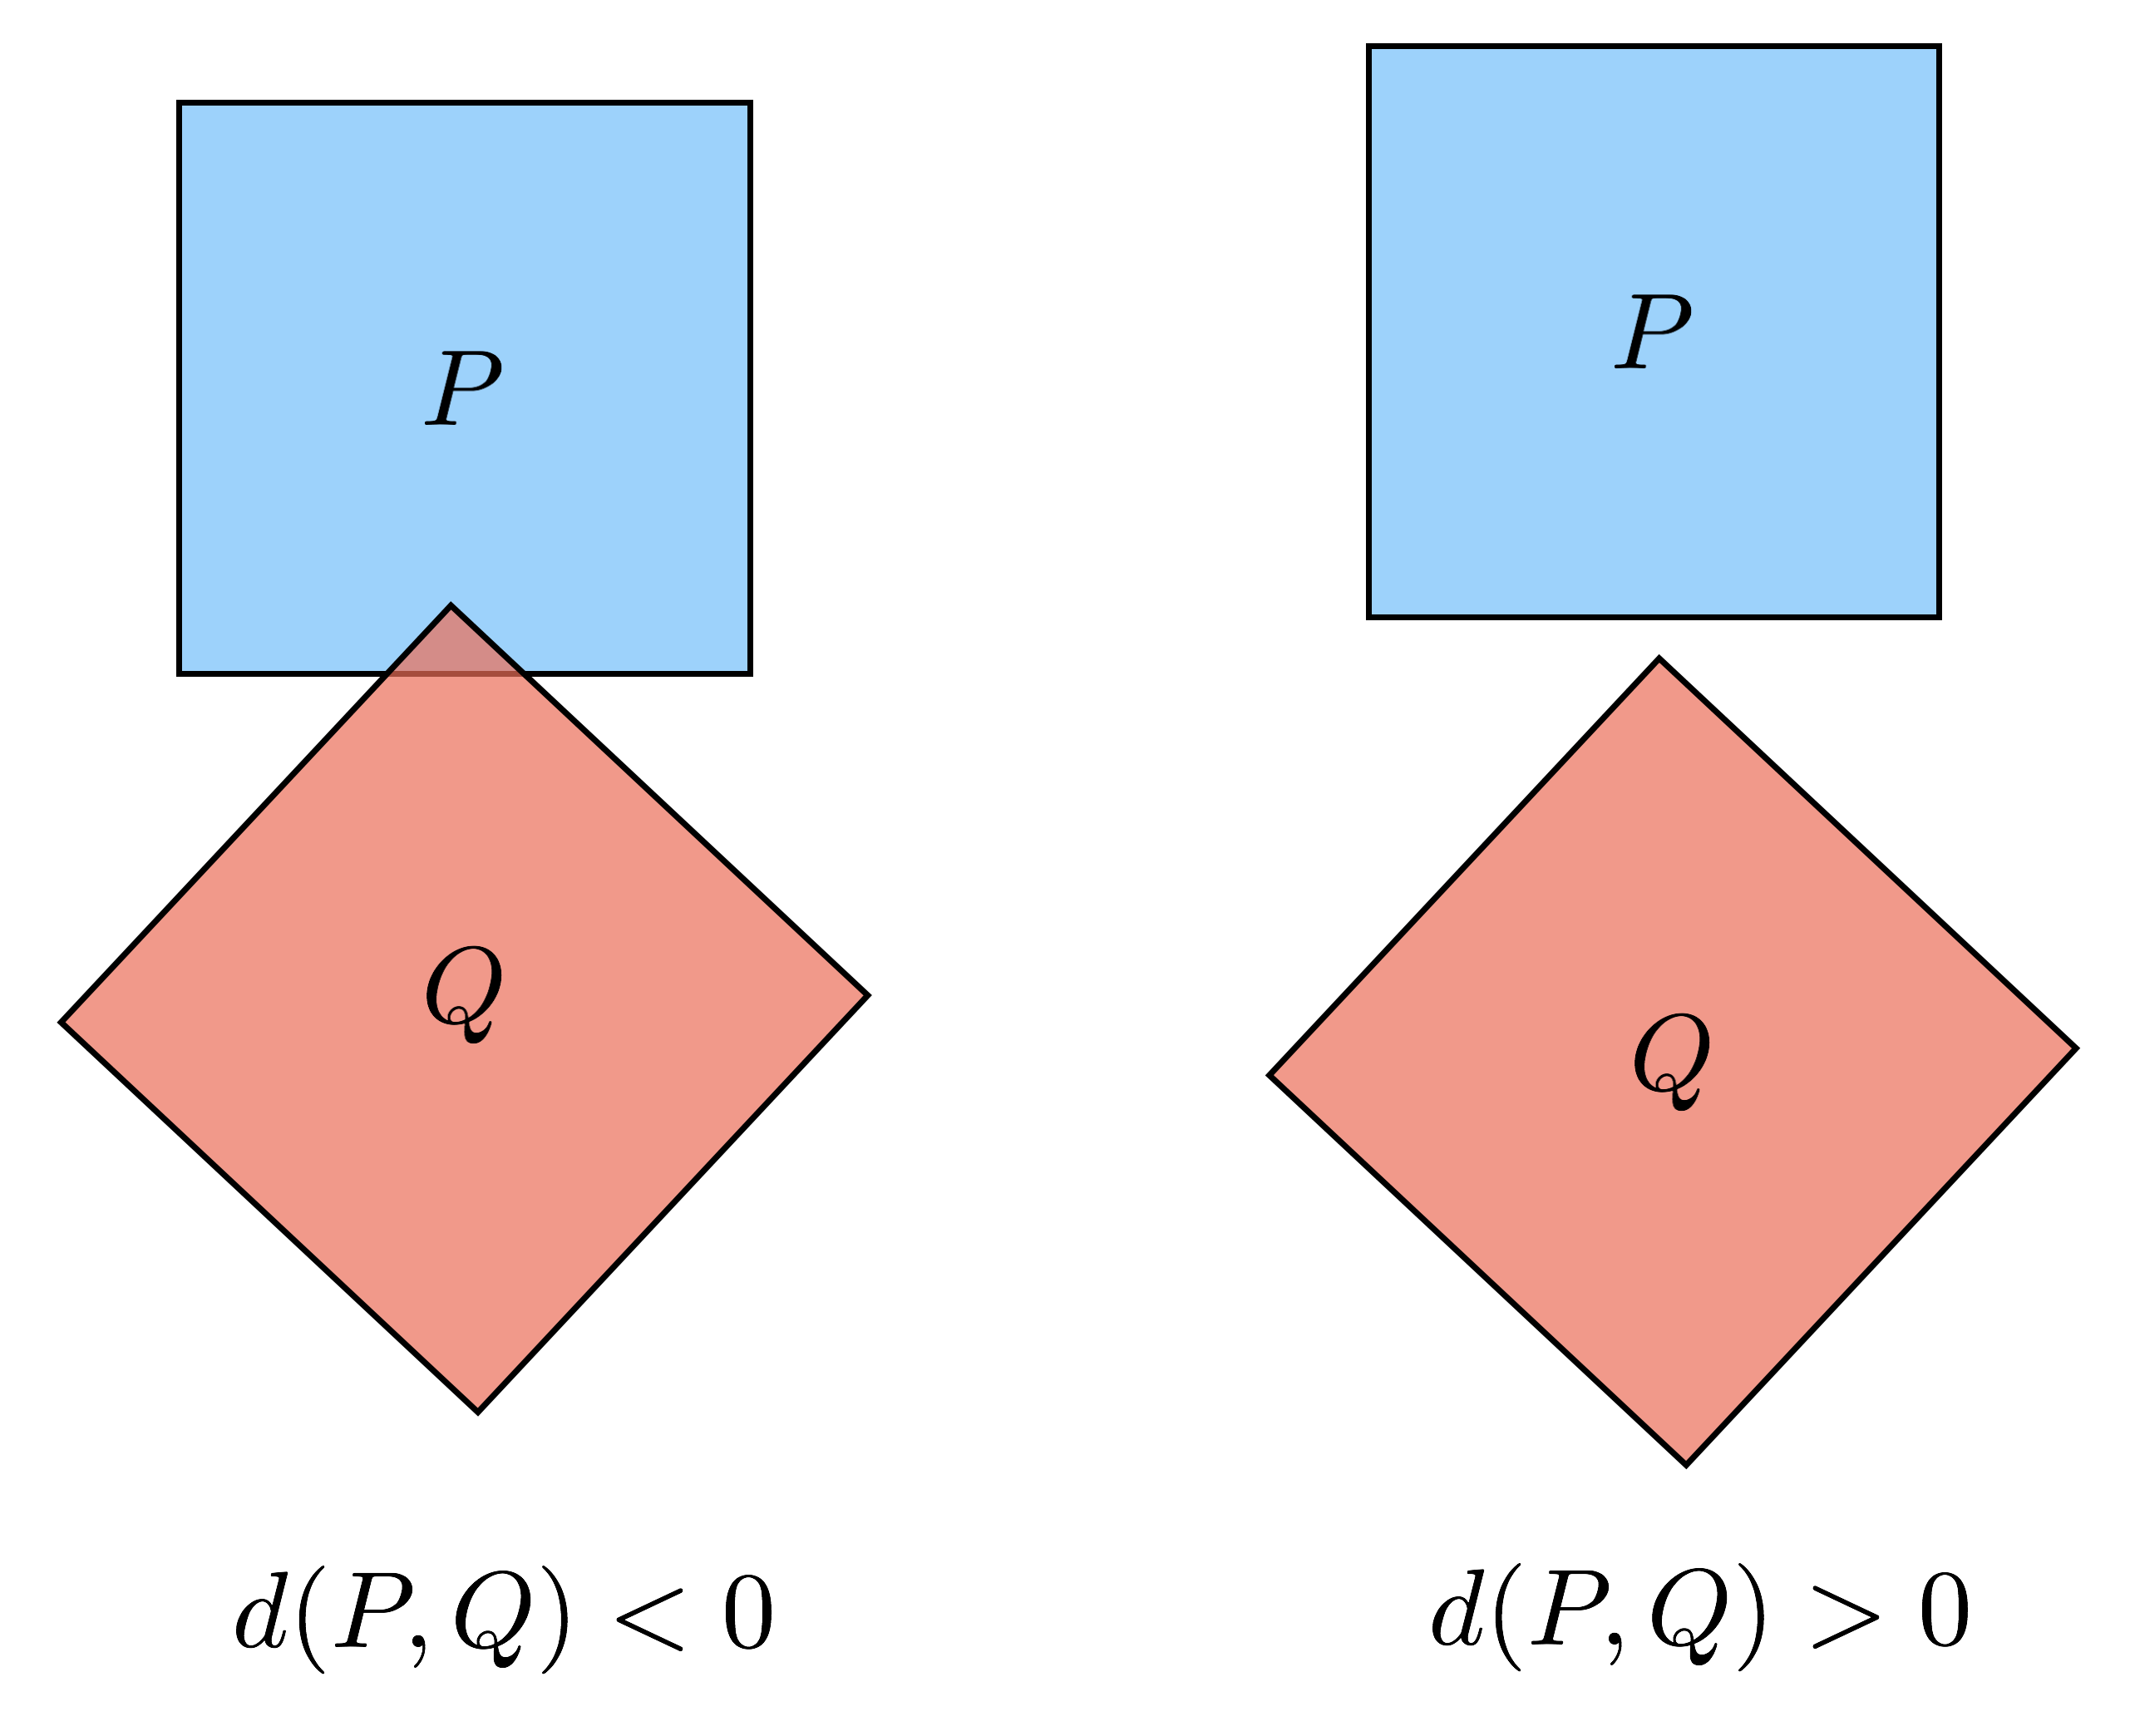
\includegraphics[width=0.5\textwidth]{ppt/signed_distance.png}
      \caption{(a) two polygons are penetrated (b) two polygons are collisional.}
      \label{fig:signed_distance}
\end{figure}
Inspired by the SAT(separated axis theorem), we always can find two points $\bp \in P, \bq \in Q$ and a normal $\bn$ which is perpendicular to one of $P$ or $Q$'s edges. The signed distance can be written as (shows in Fig:\ref{fig:distance_calculation})
\begin{equation}
	d(P, Q) = \bn^T(\bp - \bq)
	\label{eq:dPQ_first}
\end{equation}\par
\begin{figure}[!htbp]
  \centering
    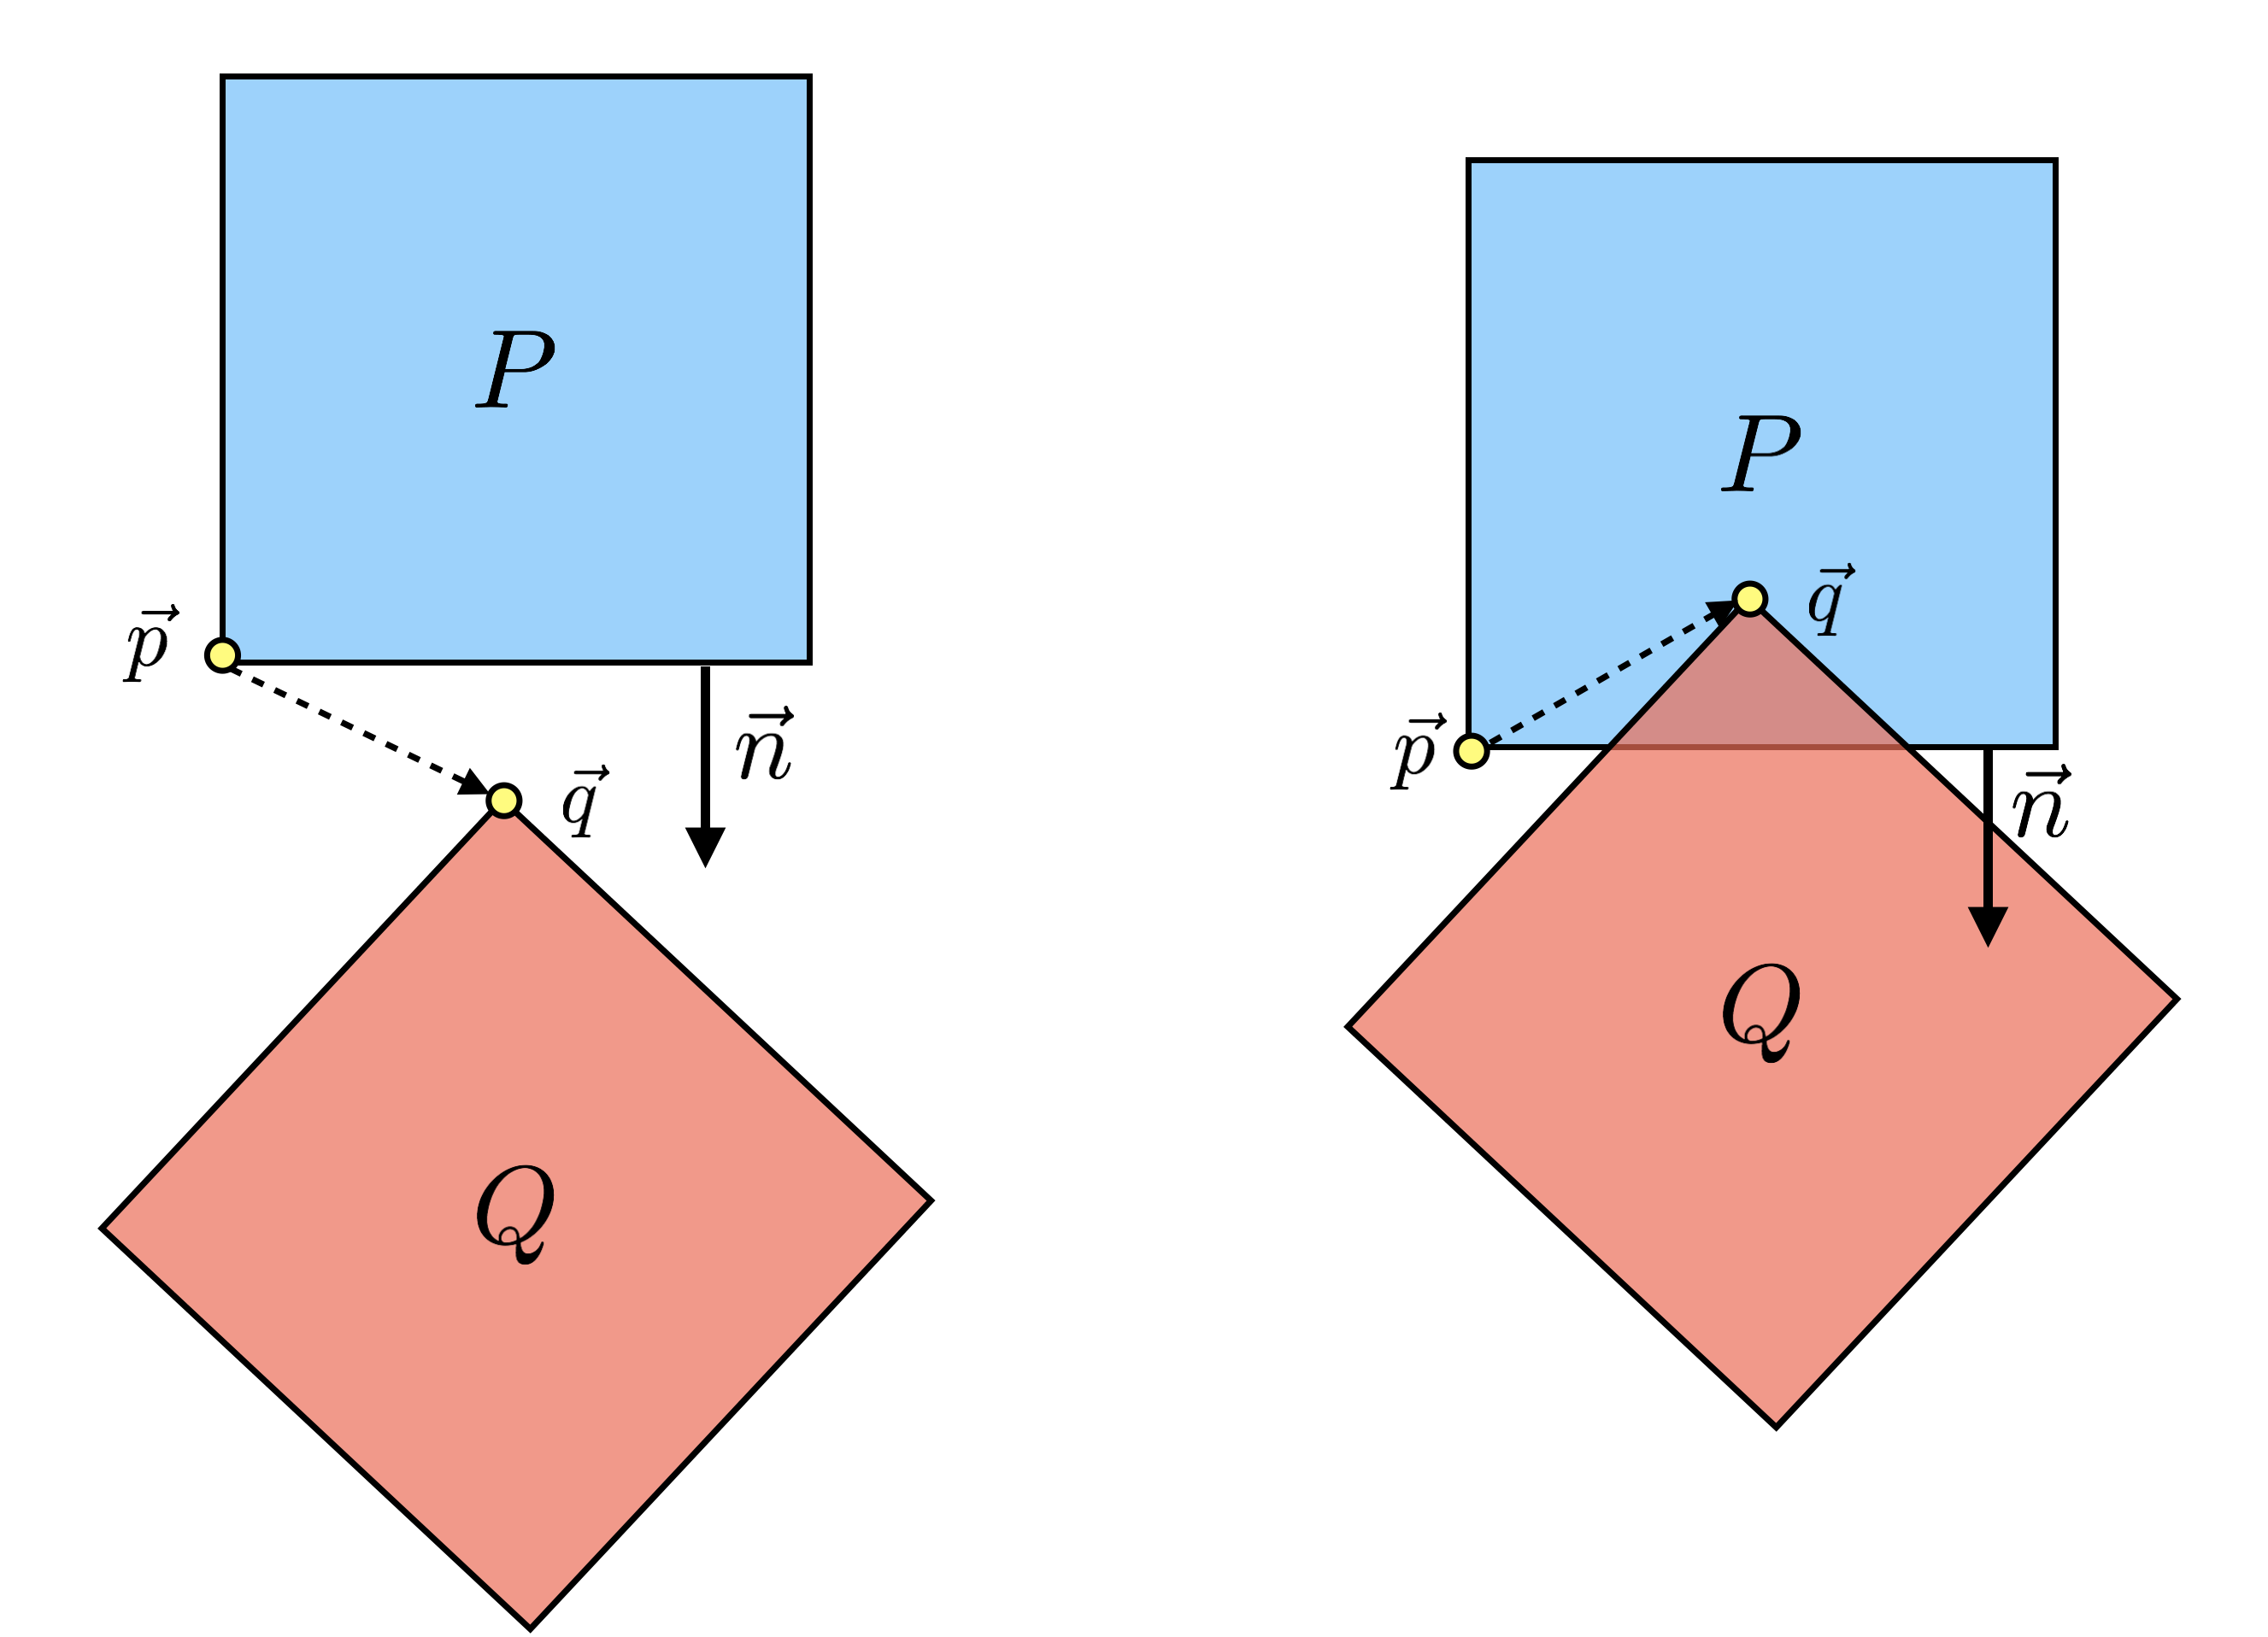
\includegraphics[width=0.5\textwidth]{ppt/distance_calculation.png}
      \caption{$\bp, \bq, \bn$ when two polygons are separated or collisional}
      \label{fig:distance_calculation}
\end{figure}
Since $P, Q$ are movable polygons during optimization, we have to express $d(P, Q)$ as a function of their translation and rotation. Let us denote $\bv^P = (\theta^P, x^P, y^P)$ and $\bv^Q = (\theta^Q, x^Q, y^Q)$ are $P, Q$'s status variable. Then Eq.\ref{eq:dPQ_first} is transformed as:
\begin{equation}
	d(P(\bv^P), Q(\bv^Q)) = \bn(\bv^P, \bv^Q)^T(\bp(\bv^P) - \bq(\bv^Q))
\end{equation}
Pleased note that $\bn(\bv^P, \bv^Q), \bp(\bv^P), \bq(\bv^Q)$ may change rapidly due to the un-smoothness of $P, Q$'s face. In order to simplify the optimization, we approximate each $\bn(\bv^P, \bv^Q), \bp(\bv^P), \bq(\bv^Q)$ locally. We assume that these variables won't change dramatically within their tiny neighbor.\par
Thus, the signed distance $d(P(\bv^P), Q((\bv^Q))$ can be linearized as:
\begin{equation}
	d(P(\bv^P), Q((\bv^Q)) \approx d(P(\bv^P_0), Q((\bv^Q_0))+ Jd(P(\bv^P_0), Q((\bv^Q_0))\begin{bmatrix}
		(\bv^P - \bv^P_0)^T \\
		(\bv^Q - \bv^Q_0)^T
	\end{bmatrix}
	\end{equation}
More specifically, Let suppose $n$ is perpendicular to one of P's edges. and
\begin{align}
	\bp(\bv^P)  &= \begin{bmatrix}
	\cos(\theta^P) & -\sin(\theta^P)\\
	\sin(\theta^P) & \cos(\theta^P)
	\end{bmatrix}(\bp -\tp) + \begin{bmatrix}
	x^P\\
	\label{eq:p_transformation}
	y^P
	\end{bmatrix} +\tp \\
	\bq(\bv^Q)  &= \begin{bmatrix}
	\cos(\theta^Q) & -\sin(\theta^Q)\\
	\sin(\theta^Q) & \cos(\theta^Q)
	\end{bmatrix}(\bq -\tq) + \begin{bmatrix}
	x^Q\\
	y^Q
	\end{bmatrix} +\tq
	\label{eq:q_transformation}
\end{align}
	
where $\bp, \bq$ is the position of $\bp(\bv^P), \bq(\bv^Q)$ when optimization starts. And $\tp, \tq$ are the central points of the polygons $P, Q$. if denote the rotation matrix in Eq.\ref{eq:p_transformation} and \ref{eq:q_transformation} as $R_{\theta^P}, R_{\theta^Q}$. \\
Then the $d(P,Q)$ can be expressed as:
\begin{align}
	d(P,Q)& =  \bn(\bv^P)^T(\bp(\bv^P) - \bq(\bv^Q))\\
			   &= \bn(\bv^P)^T[R_{\theta^P}(\bp -\tp)+\begin{bmatrix}
	x^P\\
	y^P
	\end{bmatrix} +\tp - R_{\theta^Q}(\bq -\tq) - \begin{bmatrix}
	x^Q\\
	y^Q
	\end{bmatrix} - \tq]\\
			&= f(\bv^P) + g(\bv^Q)
\end{align}
			% d(\theta, \bt) &\approx \bn^T(\bq_0 - \bp_0) +  \bn^T(R'_{\theta^0_0} \barq(\theta^0 - \theta^0_0) + \bt^0 - \bt^0_0 - R'_{\theta^1_0}(\theta^1 - \theta^1_0) \barp - \bt^1 + \bt^1_0) \\
% &= a_0 + a_1\theta^0 + a_2x^0 + a_3 y^0 + a_4\theta^1 + a_5x^1 + a_6 y^1
For $f(\bv^P)$, using Talyor expanding series:
\begin{align}
	f(\bv^P) &= \bn(\bv^P)^T(R_{\theta^P}(\bp -\tp)+\begin{bmatrix}
	x^P\\
	y^P
	\end{bmatrix} +\tp) \\
	&\approx [\bn_0 + \begin{bmatrix}
		-\bn_{0y}\\
		\bn_{0x}
	\end{bmatrix}(\theta^P - \theta^P_0)][\bp_0 + R'_{\theta^P_0}(\bp - \tp)(\theta^P - \theta^P_0) + \begin{bmatrix}
	x^P - x^P_0\\
	y^P - y^P_0
	\end{bmatrix}]
\end{align}
where $\bn_0 = \bn(\bv^P_0), p_0 = \bp(\bv^P_0)$ \\
Same in $g(\bv^Q)$:
\begin{equation}
	g(\bv^P) \approx [\bn_0 + \begin{bmatrix}
		-\bn_{0y}\\
		\bn_{0x}
	\end{bmatrix}(\theta^P - \theta^P_0)][\bq_0 + R'_{\theta^Q_0}(\bq - \tq)(\theta^Q - \theta^Q_0) + \begin{bmatrix}
	x^Q - x^Q_0\\
	y^Q - y^Q_0
	\end{bmatrix}]
\end{equation}
where $\bq_0 = \bp(\bv^P_0)$ \\
And combining these two function as:
\begin{equation}
	d(P, Q) = a_0 + a_1\theta^P + a_2x^P + a_3y^P + a_4\theta^Q + a_5x^Q + a_6y^Q
\end{equation}
The $a_i$ can be written as:
\begin{align}
				a_1 &= \bn^TR'_{\theta^P_0} (\bp - \tp) + \bn_1^T(\bp_0 - \bq_0) \\
				a_2 &= \bn_{0x} \\
				a_3 &= \bn_{0y} \\
				a_4 &= -\bn^TR'_{\theta^Q_0} (\bq - \tq) \\
				a_5 &= - \bn_{0x}  \\
				a_6 &= - \bn_{0y}  \\
				a_0 &=  (\bn_0 - \bn_1\theta^P_0)^T(\bp_0 - \bq_0) - \bn_0^TR'_{\theta^P_0} (\bp - \tp)\theta^P_0 \\
				&- \bn_0^TR'_{\theta^Q_0} (\bq - \tq) \theta^Q_0 + \bn_0^T\begin{bmatrix}
	x^Q_0 - x^P_0\\
	 y^Q_0 - y^P_0
	\end{bmatrix} 
\end{align}
where 
\begin{equation}
	\bn_1 = \begin{bmatrix}
		-\bn_{0y}\\
		\bn_{0x}
	\end{bmatrix}
\end{equation} 
\subsection{Improved signed distance}
However, only using two points $(\bp, \bq)$ to describe the signed distance may have problems when the two polygons have face in parallel. \\
\begin{figure}[!htbp]
  \centering
    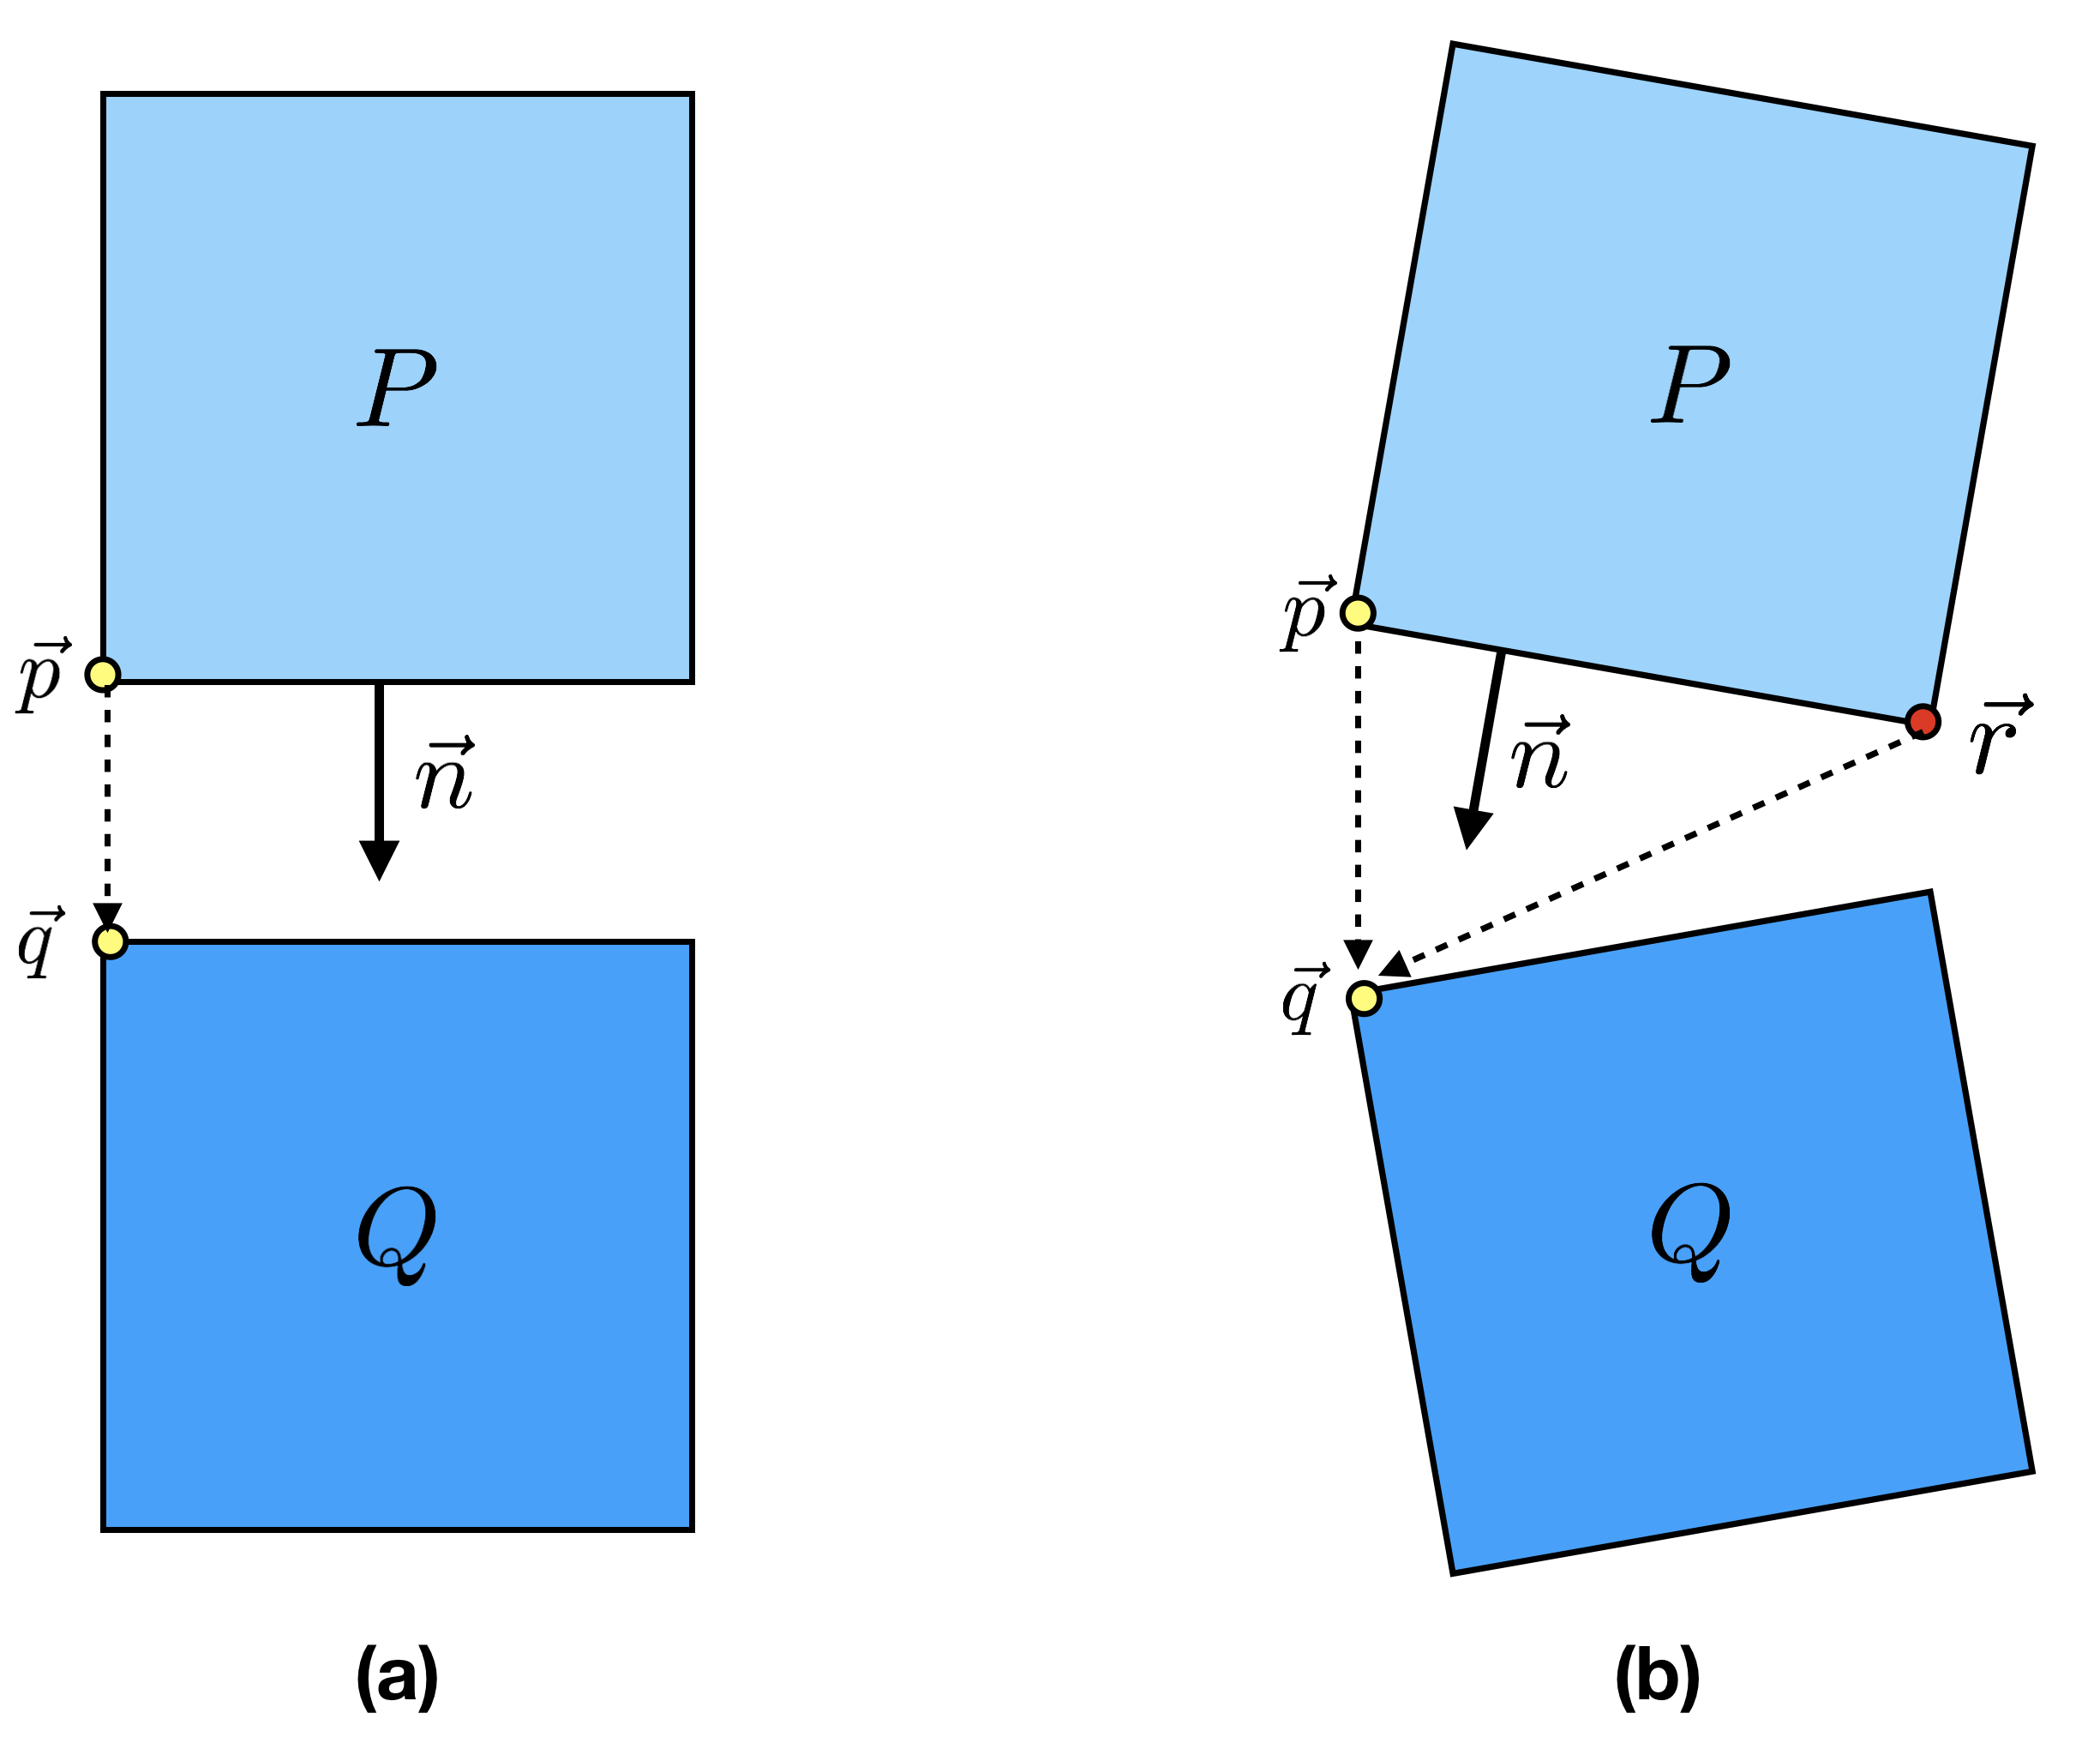
\includegraphics[width=0.5\textwidth]{ppt/problem_distance.png}
      \caption{An unapproriate approximation of signed distance when two polygons have faces in parallel.}
      \label{fig:problem_distance}
     \end{figure}
In Fig.\ref{fig:problem_distance}, the signed distance actually drop while our approximated function indicated an increase in distance. Let's denote the distance from $(\bp, \bq, \bn)$ as $d_{\bp, \bq, \bn}(P, Q)$. Then apparently in Fig.\ref{fig:problem_distance}:
\begin{equation} 
	d_{\bp, \bq, \bn}(P, Q) >  d_{\br, \bq, \bn}(P, Q)
\end{equation}
To resolve this problem, we use two pairs of $(\bp, \bq), (\br, \bq)$ to approximate the $d(P, Q)$:
\begin{align} 
	d(P, Q)   = \min(d_{\bp, \bq, \bn}(P, Q) , d_{\br, \bq, \bn}(P, Q))
\end{align}
\subsection{Collision resolve} 
\end{document}